
\documentclass[tikz,convert={convertexe={magick.exe}}]{standalone}
\usetikzlibrary{arrows.meta, shapes}

\begin{document}
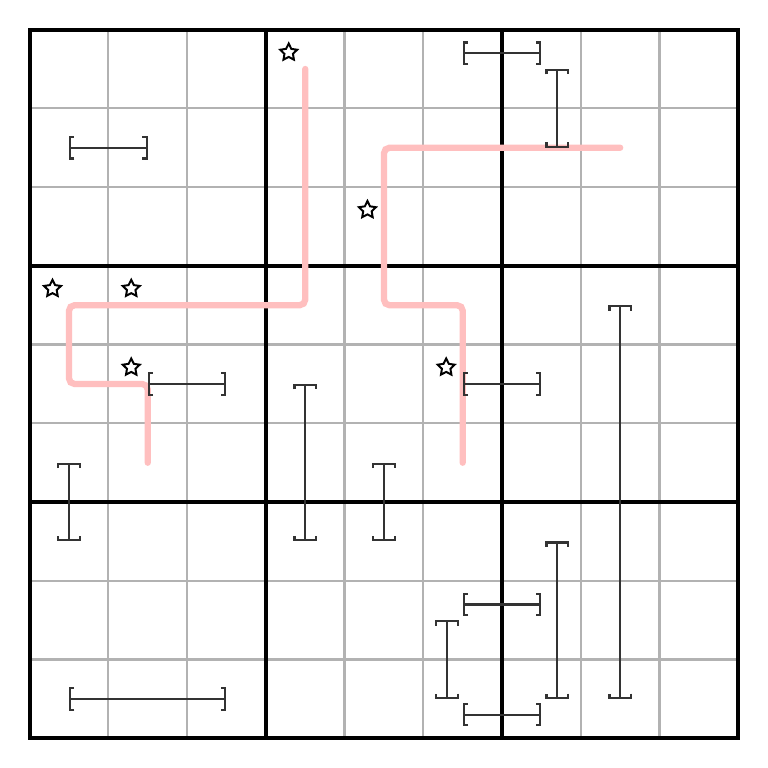
\begin{tikzpicture}
[int/.style={color=black!80,thick, {Bracket[width=3mm]}-{Bracket[width=3mm]}},
snake/.style={color=pink,line width=0.8mm, line cap=round, rounded corners=0.7mm},
fp/.style={inner sep=0.8mm, star point ratio=0.5, line width=0.25mm, draw=black, fill=white, star, star points = 5, rounded corners = 0mm, rotate=180, xshift=0.21cm, yshift=-0.21cm}]
\fill[color=white] (0,0) rectangle (9,9);
\draw[thick, color=gray!60] (0,0) grid (9,9);
\draw[step=3, color=black, very thick] (0,0) grid (9,9);
\draw[color=black, line width=0.5mm] (0,0) rectangle (9,9);


\draw[snake] (1.5,3.5) --++(0,1) node[fp]{} --++(-1,0) --++(0,1) node[fp]{} --++(1,0) node[fp]{} --++(2,0) --++(0,3) node[fp]{};
\draw[snake] (5.5,3.5) --++(0,1) node[fp]{} --++(0,1) --++(-1,0) --++(0,1) node[fp]{} --++(0,1) --++(3,0);

\draw[int] (0.5,0.5) --++(2,0);

\draw[int] (5.5,0.3) -- (6.5,0.3);
\draw[int] (5.3,0.5) --++(0,1);
\draw[int] (5.5,1.7) -- (6.5,1.7);
\draw[int] (6.7,0.5) --++(0,2);

\draw[int] (0.5,2.5) --++(0,1);
\draw[int] (0.5,7.5) --++(1,0);

\draw[int] (5.5,8.7) -- (6.5,8.7);
\draw[int] (6.7,7.5) --++(0,1);

\draw[int] (5.5,4.5) --++(1,0);
\draw[int] (7.5,0.5) --++(0,5);

\draw[int] (1.5,4.5) --++(1,0);
\draw[int] (3.5,2.5) --++(0,2);
\draw[int] (4.5,2.5) --++(0,1);

\end{tikzpicture}
\end{document}